\section{Introduction}
\label{sec:introduction}

\glsresetall

% \textbf{What is the problem? Why graph network simulators?}
Physics simulation is central to engineering disciplines ranging from structural mechanics to robotics, yet classical solvers based on the finite element method are computationally expensive \citep{zienkiewicz2005finite,stanova2015finite}.
\glspl{gns} have emerged as fast and differentiable surrogates for mesh-based physics, offering orders-of-magnitude speedups over classical solvers~\citep{battaglia2016interaction, pfaff2020learning, brandstetter2021message, linkerhagner2023grounding, wurth2025diffusion}.
However, standard \glspl{gns} assume known process conditions, resulting in a parameter estimation problem when physical parameters change.
Classical system identification can recover such parameters, but doing so per-instance multiplies the experimental and computational cost in ways that scale poorly~\citep{aastrom1971system, lennart1999system, isakov2006inverse, wu2015galileo, murthy2020gradsim, antonova2023rethinking}.
Test-time gradient inversion through a differentiable simulator is one response, but reintroduces a per-instance optimization loop and there is no guarantee that the loss objective for inversion is well-conditioned~\citep{qzhao2022graphpde, wang2024latent}.
In-context conditioning instead amortizes identification by encoding a set of context trajectories into a latent material descriptor, enabling rapid adaptation to new material configurations at inference time~\citep{dahlinger2025mango}.
In this work, we formulate adaptive physical simulation as a real-to-sim in-context learning problem, in which a novel spatio-temporal encoder infers a latent description of the unknown physical properties from point cloud observations and provides it as context to the simulator.

% \textbf{Why point clouds? What are the benefits and challenges?}
Operating on meshes instead of points~\citep{robocook23, hd-vpd} helps \glspl{gns} generate stable and more accurate predictions over long sequences.
However, mesh trajectories of arbitrary deforming objects are not directly observable with standard sensing; reconstructing them requires either invasive marker setups or template registration that itself depends on geometric and constitutive priors~\citep{MansourZK24,LoperMB14}.
Point clouds, in contrast, are produced directly by depth cameras and LiDAR and capture 3D geometry of deforming objects.
Because they rely on geometric structure rather than surface appearance, sim-to-real transfer is less constrained by rendering fidelity~\citep{dexpoint, 3DDA, adapt3r, pointmappolicy}.
While point cloud observations can easily be generated from meshes, point clouds from the real world do not contain correspondences between points from subsequent time steps.
This complicates the estimation of physical parameters, since the motion of individual points contains the most information about those parameters.
Unlike in mesh-based approaches, these correspondences must be inferred indirectly.


% \textbf{Par 1 — Problem framing}
% %
% While simulators are central to engineering design, their predictive accuracy depends on physical parameters that are rarely known precisely for any given real-world scenario. \citep{landau2012theory, blazek2015computational}
% These parameters vary across instances and drift over time: batch-to-batch variation, tooling wear, thermal aging, and chemical curing can all change effective stiffness or viscosity, sometimes within a single production run. \citep{TODO}
% Classical system identification can recover such parameters, but doing so per-instance — once for every new batch, every drift event, every new geometry — multiplies experimental and computational cost in ways that scale poorly with deployment frequency~\citep{aastrom1971system, lennart1999system, isakov2006inverse, wu2015galileo, murthy2020gradsim, antonova2023rethinking}.
% This motivates an alternative: amortize material identification across instances, so that adapting to a new configuration requires only observation of that configuration, not a fresh optimization.

% \textbf{Par 2 — Why existing approaches fall short}
% %
% \glspl{gns} have emerged as fast, differentiable surrogates for mesh-based physics, offering orders-of-magnitude speedups over classical solvers. \citep{battaglia2016interaction, pfaff2020learning, brandstetter2021message, linkerhagner2023grounding, wurth2025diffusion}
% However, standard \glspl{gns} assume known process conditions and inherit the parameter-estimation problem when these conditions change.
% Test-time gradient inversion through a pretrained simulator is one response, but reintroduces a per-instance optimization loop and demands surrogates that remain well-conditioned for inversion. \citep{qzhao2022graphpde, wang2024latent}
% In-context conditioning instead amortizes identification by encoding a set of context trajectories into a latent material descriptor, sidestepping test-time optimization. \citep{dahlinger2025mango}
% However, mesh trajectories of arbitrary deforming objects are not directly observable with standard sensing — recovering them requires either invasive marker setups, template registration that itself depends on geometric and constitutive priors, or running a calibrated simulator. \citep{TODO}
% Point clouds, by contrast, are produced directly by depth cameras and LiDAR, and capture 3D geometry of deforming objects without requiring view-consistent rendering or learned correspondences.
% Point cloud observations can be easily generated from meshes.
% Point clouds place the focus on geometry rather than color/texture, making sim2real easier.

\begin{figure}[t]
    \centering
    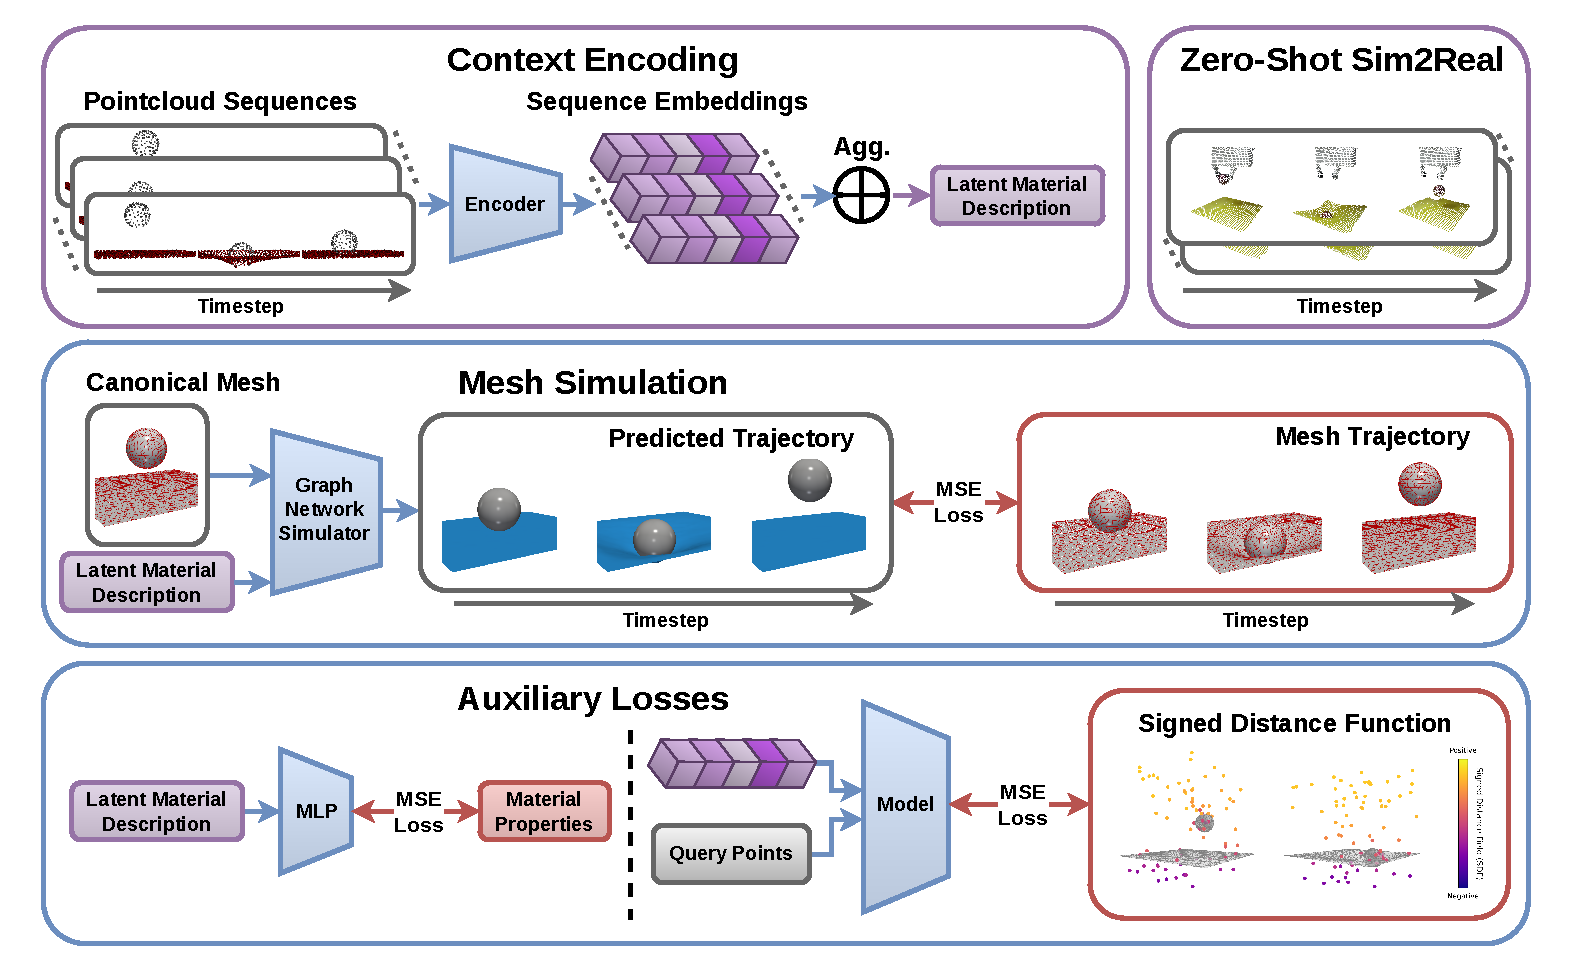
\includegraphics[width=\textwidth]{figures/peach_fig1_v4.pdf}
    \caption{
    Overview of the \acrfull{peach} framework.
    Point cloud sequences from several simulated or real trajectories are encoded into a single latent material description via our novel spatio-temporal encoder architecture.
    The aggregated latent vector conditions a mesh-based simulator, which predicts complete trajectories from an initial mesh.
    % The method is trained to minimize the average simulation error, and uses an auxiliary loss on the latent material description to ensure physical consistency.
    To improve accuracy, we apply auxiliary losses based on the ground truth physical properties and the Signed Distance Field (SDF).
    % It additionally to predict full mesh dynamics, and is also used to predict material properties via an auxiliary MLP; both predictions are supervised during training. 
    During inference, only the context point cloud sequences and an initial geometry are needed to simulate behavior with novel, unseen material properties.
    }
    \vspace{-0.3cm}
    \label{fig:overview}
\end{figure}

% \textbf{Our method}
To address these challenges, we introduce \glsf{peach}, an in-context framework that conditions a graph network simulator on a small set of observed point cloud sequences.
This framework is able to predict mesh-level dynamics for unseen materials, without any test-time parameter optimization.
\gls{peach} extends the conditional neural process framework \citep{garnelo_conditional_2018} to spatio-temporal observations: a spatio-temporal encoder maps each point cloud sequence to a latent vector, and the resulting set is aggregated into a single material descriptor that conditions the simulator.
Our novel encoder architecture extends the common point-patch paradigm~\citep{pointMAE, pointBERT, pointGPT} by treating a sequence as a single point cloud embedded in 4D space-time.
By relying on proximity in 4D space-time, the network can extract physical properties from the observation without explicit point-to-point correspondences.
% We pair this encoder with a trajectory-level simulator that predicts entire rollouts in a single forward pass, avoiding the train-test mismatch of autoregressive methods, which are trained on single-step predictions but deployed over long horizons, leading to compounding errors~\citep{egno2024, dahlinger2025mango}.
% Training the encoder–simulator stack end-to-end additional supervision: we found in preliminary experiments that the latent material descriptor is otherwise under-constrained \todo{forward-ref the ablation}.
While this architecture is already competitive, we found in preliminary experiments that additional auxiliary losses can further improve the results.
We investigate two auxiliary losses applied during training only: a regression head that grounds the latent embedding in the ground truth physical parameters, and a \gls{sdf} reconstruction loss that encourages the encoder to retain fine-grained geometric information in the earlier layers.
%prevents the encoder from collapsing context information into a representation that fits the regression target but discards scene-level signal.
For inference, the model receives an initial mesh of the canonical geometry, which is typically available from CAD or a one-time scan, and $1$ to $8$ point cloud sequences from the target process. \gls{peach} predicts the remaining mesh simulation using the implicit physical properties defined by the context.

% \textbf{Par 3 — Our method, PEACH}
% %
% We introduce \gls{peach}, an in-context framework that conditions a graph network simulator on a small set of observed point cloud sequences to predict mesh-level dynamics for unseen materials, without any test-time parameter optimization.
% \gls{peach} extends the conditional neural process framework to spatio-temporal observations: a spatio-temporal encoder maps each context sequence to a latent vector, and the resulting set is aggregated into a single material descriptor that conditions the simulator. \citep{garnelo_conditional_2018} \todo{tie back to in-context conditioning in Par 2}
% We pair this encoder with a trajectory-level simulator that predicts entire rollouts in a single forward pass, which both stabilizes training relative to autoregressive backpropagation through long horizons and pairs naturally with the encoder's single sequence-level descriptor. \citep{egno2024, dahlinger2025mango}
% The encoder operates on 4D space-time point clouds via farthest-point sampling and a transformer backbone, designed to extract material-relevant features from sequences without point correspondences across time~\citep{Gyenes24}.
% Training the encoder–simulator stack end-to-end requires additional supervision: we found in preliminary experiments that the latent material descriptor is otherwise under-constrained \todo{forward-ref the ablation}.
% We therefore apply two auxiliary losses during training only: a material-parameter regression head that grounds the descriptor in known physical quantities, and a signed-distance-field reconstruction loss that prevents the encoder from collapsing context information into a representation that fits the regression target but discards scene-level signal. \citep{TODO}
% At inference, the user supplies an initial mesh of the canonical geometry - typically available from CAD or a one-time scan - and 1-8 point cloud sequences from the target process.


% \textbf{Contributions}
To summarize, our contributions are as follows:
(i) We propose \gls{peach}, an end-to-end architecture that efficiently and accurately simulates a mesh-based trajectory conditioned on a handful of observed point clouds, without test-time optimization.
As a  key benefit, our novel spatio-temporal point cloud encoder is applicable to any operation on point cloud sequences due to its generality.
(ii) We demonstrate \gls{peach}'s sim-to-real capability through one-shot, rapid adaptation of a real-world scene in which a robot drops a ball onto a rubber trampoline, a setting beyond the reach of mesh-based methods.
We additionally validate on four simulation scenes featuring deformable objects and outperform baselines with access to the ground truth context mesh.
(iii) Through parameter studies, we provide insights that underscore the necessity of auxiliary losses for parameter regression and \gls{sdf}.
Furthermore, we visualize the latent space and show statistically that it converges with increasing context size at a rate close to averaging independent observations, and that distances between tasks in the latent space strongly correlate with distances between their physical parameters.


\begin{figure}[t]
    \centering
    \begin{minipage}{0.2\textwidth}
        \centering
        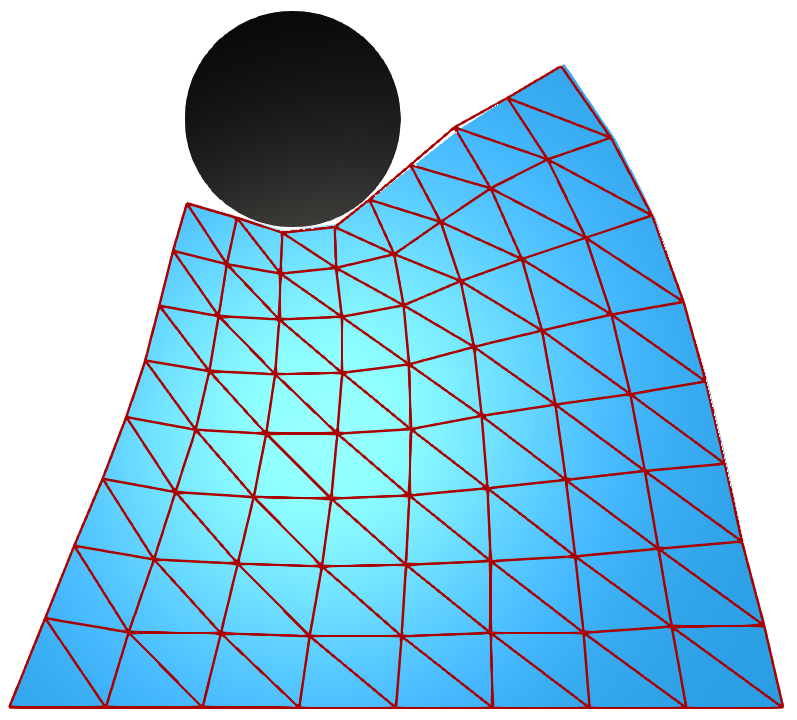
\includegraphics[width=\textwidth]{figures/task_overview_data/db.png}
    \end{minipage}
    \hspace{1mm}
    \begin{minipage}{0.29\textwidth}
        \centering
        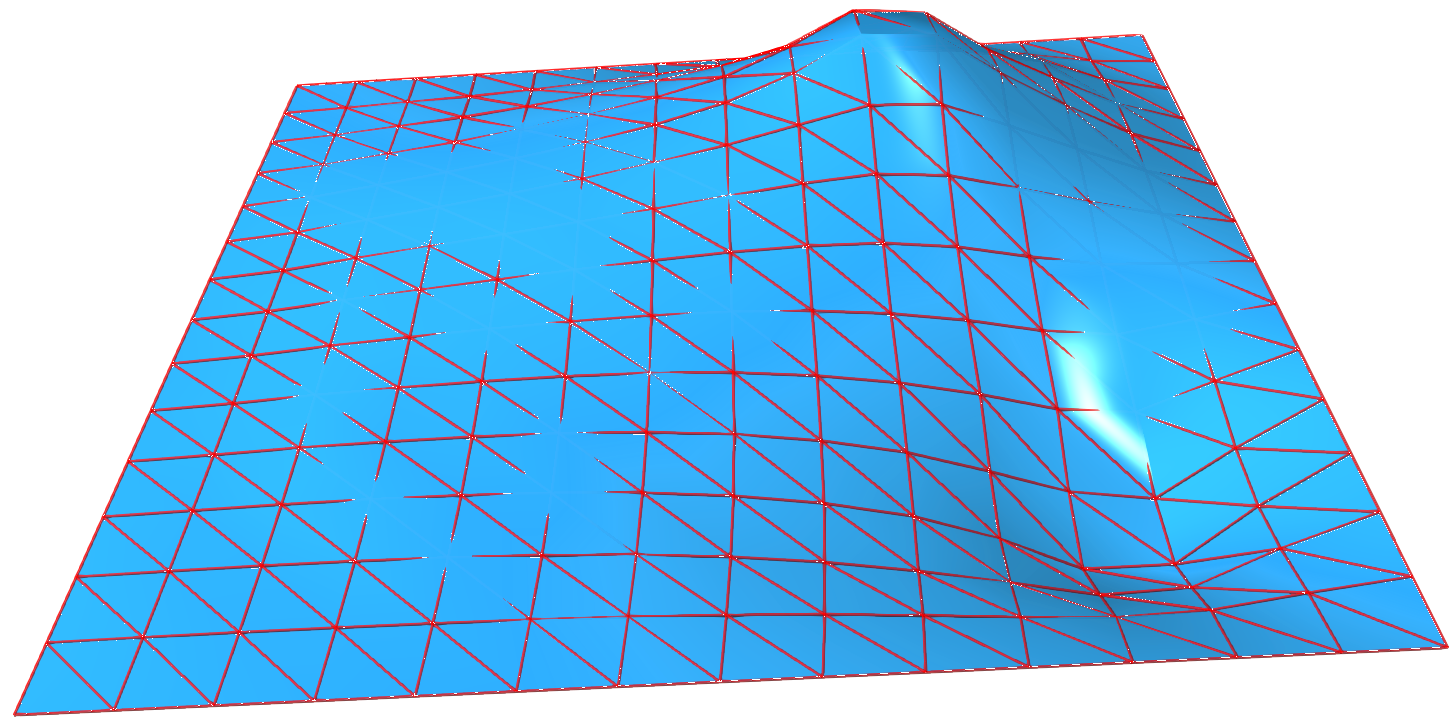
\includegraphics[width=\textwidth]{figures/task_overview_data/sd.png}
    \end{minipage}
    \begin{minipage}{0.48\textwidth}
        \centering
        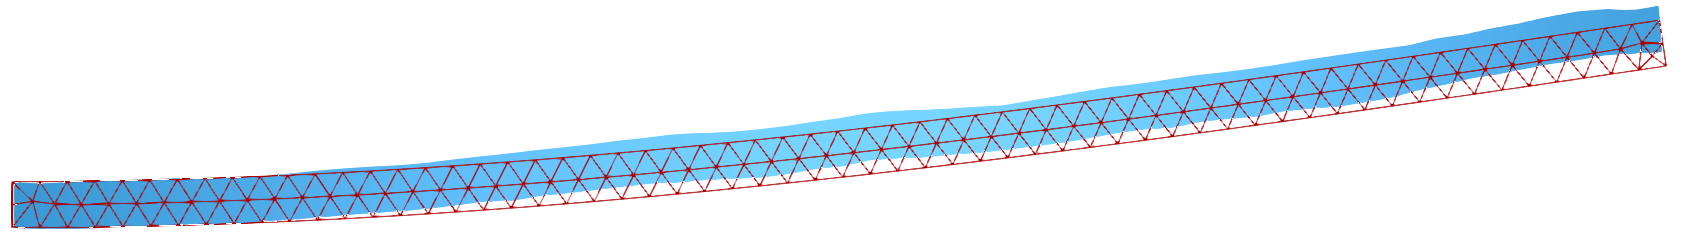
\includegraphics[width=\textwidth]{figures/task_overview_data/bbv.png}
    \end{minipage}%
\vspace{0.05mm}

    \begin{minipage}{0.2\textwidth}
        \centering
        {\small \texttt{Deforming Block}}
    \end{minipage}
    \begin{minipage}{0.29\textwidth}
        \centering
        {\small \texttt{Sheet Deformation}}
    \end{minipage}
    \begin{minipage}{0.48\textwidth}
        \centering
        {\small \texttt{Bending Beam}}
    \end{minipage}%
\vspace{-5mm}

    \begin{minipage}{\textwidth}
        \centering
        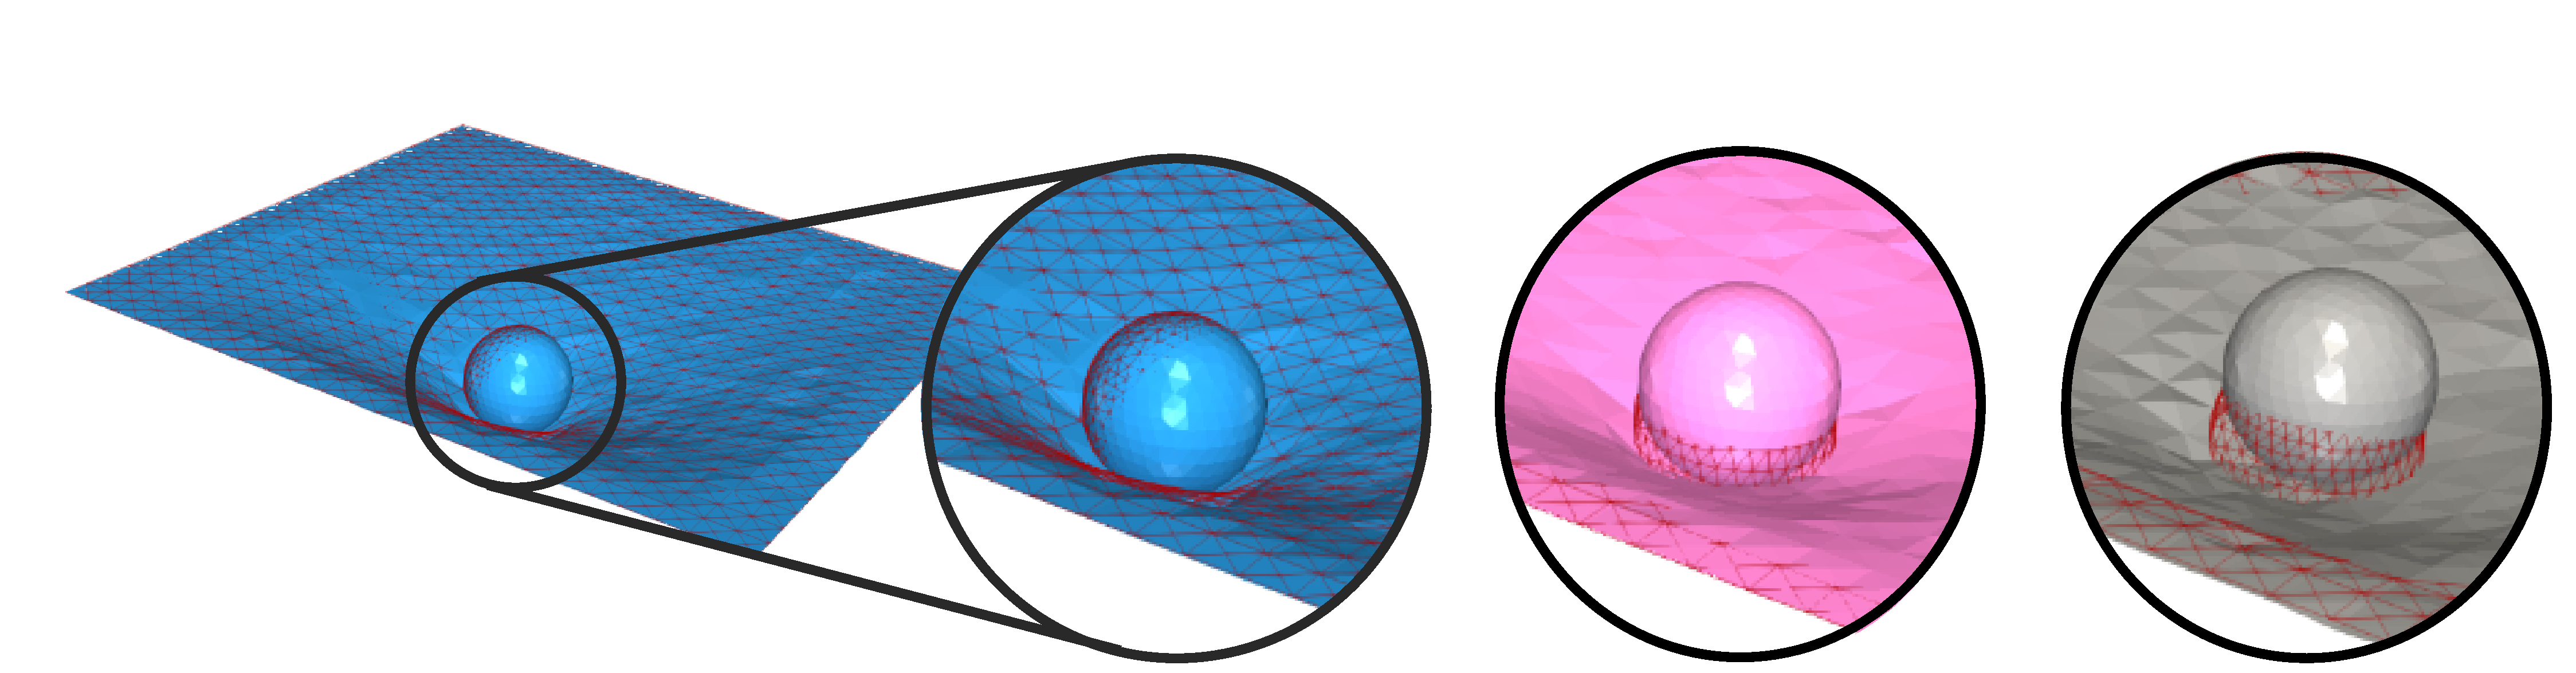
\includegraphics[width=\textwidth, trim={50 0 0 0}, clip]{figures/task_overview_data/task_overview.pdf}
    \end{minipage}

    % \begin{minipage}{0.325\textwidth}
    %     \centering
    %     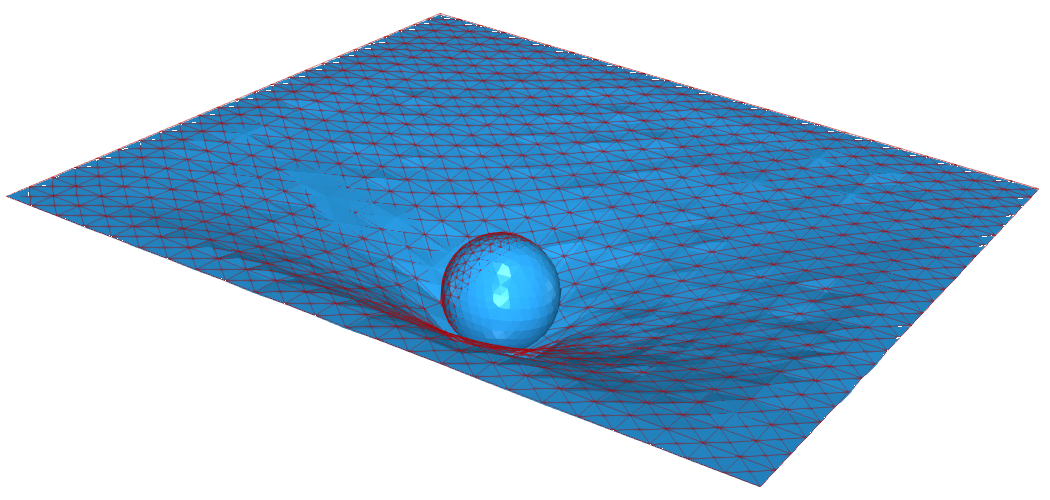
\includegraphics[width=\textwidth]{figures/task_overview_data/trampoline_peach.png}
    % \end{minipage}
    % \begin{minipage}{0.325\textwidth}
    %     \centering
    %     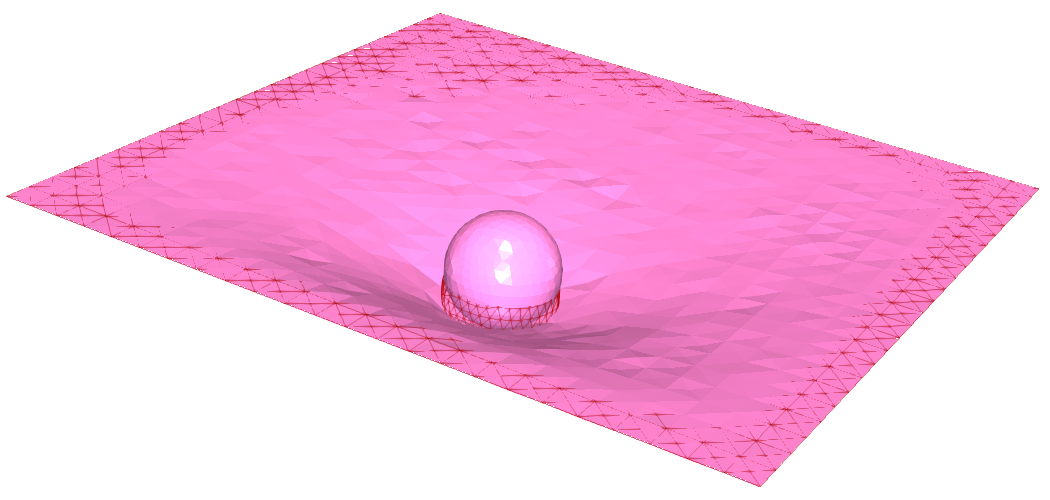
\includegraphics[width=\textwidth]{figures/task_overview_data/trampoline_pstnet.png}
    % \end{minipage}
    % \begin{minipage}{0.325\textwidth}
    %     \centering
    %     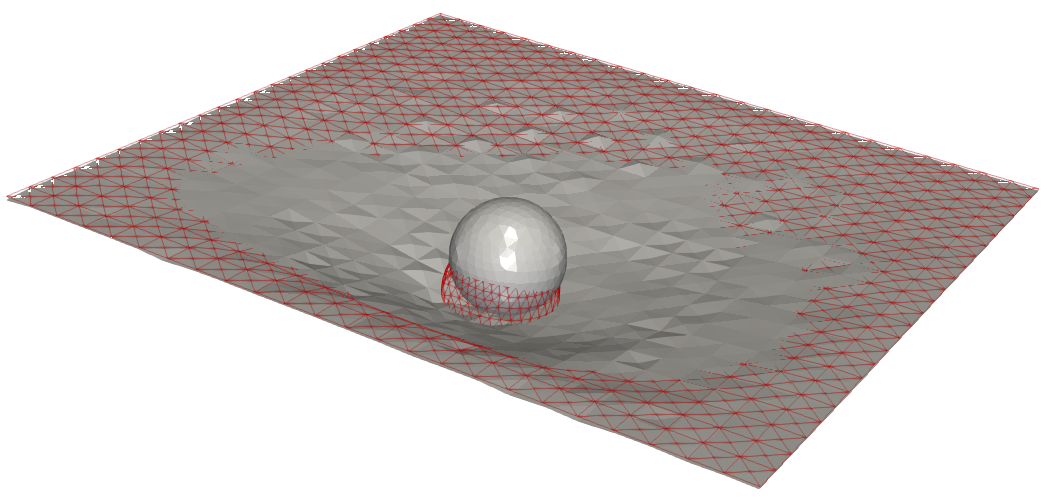
\includegraphics[width=\textwidth]{figures/task_overview_data/trampoline_dummy.png}
    % \end{minipage}%
    % \vspace{0.05mm}
    
    \begin{minipage}{0.3\textwidth}
        \centering
        {\small \texttt{Trampoline }}
    \end{minipage}
    \begin{minipage}{0.2\textwidth}
        \centering
        {\small \hspace{0.6cm} \textit{PEACH}}
    \end{minipage}
    \begin{minipage}{0.23\textwidth}
        \centering
        {\small \hspace{0.8cm}\textit{PSTNet Encoder}}
    \end{minipage}
    \begin{minipage}{0.23\textwidth}
        \centering
        {\small \hspace{0.5cm} \textit{No Context}}
    \end{minipage}
    


\caption{
    Overview of the four simulation scenes.
    The environments cover a range of deformable object types and material models, from purely elastic to viscoelastic constitutive behaviors, with varying material properties across tasks.
    Qualitative predictions of \gls{peach} and selected baselines are shown in \textcolor{blue}{blue}, \textcolor{TabPink}{pink}, and \textcolor{gray}{gray}, respectively, with ground-truth meshes overlaid in \textcolor{red}{red}.
}
\vspace{-0.6cm}
\label{fig:task_overview}
\end{figure}


% \textbf{Par 4 — Results}
% %
% Our headline result is a real-world deformation experiment in which a robot drops balls of varying mass and stiffness onto a deformable sheet of unknown material; \gls{peach} predicts the resulting deformation \todo{quantitative anchor: e.g., within X mm RMSE, or matching per-instance optimization at a fraction of the cost} from only a few reference trajectories, in a single forward pass and without any per-instance optimization.
% On four simulated deformation benchmarks \todo{name datasets} \citep{dahlinger2025mango}, \gls{peach} matches a strong mesh-based reference (MaNGO) that has access to ground-truth mesh trajectories, and outperforms point cloud baselines including PSTNet \citep{fan2021pstnet} and a spatio-temporal GNN encoder.
% Ablations confirm that both auxiliary losses contribute to final accuracy, and an analysis of the latent space shows that the learned material descriptors \todo{state precise finding once known: e.g., linearly decode Young's modulus with R² = X}.

% \textbf{Par 5 — Contributions}
% %
% (i) We formulate adaptive physical simulation as a real-to-sim in-context learning problem from point cloud sequences, and identify the sensing requirements that have prevented mesh-context approaches from applying to real settings.
% (ii) We propose \gls{peach}, an end-to-end architecture pairing a 4D spatio-temporal point cloud encoder with a trajectory-level GNS, regularized by material-regression and SDF auxiliary losses.
% (iii) We validate \gls{peach} on four simulated deformation benchmarks, where it matches mesh-based references that use strictly more information, and on a real-world robot-sheet interaction task, where it produces accurate deformation predictions in a single forward pass from a handful of point cloud trajectories.


% Simulating complex physical systems is fundamental to engineering disciplines ranging from structural mechanics~\citep{landau2012theory} to fluid dynamics~\citep{blazek2015computational}. 
% Traditional mesh-based methods, such as the \gls{fem}~\citep{brenner2008mathematical, reddy2019introduction}, provide high precision, but quickly become computationally expensive.
% These methods also rely on precise knowledge of physical parameters, such as stiffness or density, which are frequently unknown in practice.
% Deep learning-based surrogates, particularly \glspl{gns}~\citep{battaglia2016interaction, pfaff2020learning, brandstetter2021message, linkerhagner2023grounding, wurth2025diffusion}, have emerged as a promising alternative that offers orders-of-magnitude speedups and inherent differentiability. 
% \glspl{gns} handle physical data by modeling arbitrary entities and their relations as a graph. 
% Standard \glspl{gns} typically learn to evolve a given input mesh over time for known process conditions. 
% However, they rely on expensive system identification methods~\citep{aastrom1971system, lennart1999system, isakov2006inverse, wu2015galileo, murthy2020gradsim, antonova2023rethinking}. for parameter estimation when process conditions, such as the material parameters, change.
% \todo{expand a bit}

% While some methods use gradient-based inversion on pre-trained simulators to estimate parameters~\citep{qzhao2022graphpde, wang2024latent}, these require computationally expensive optimization loops at test time.
% Recently, \gls{mango}~\citep{dahlinger2025mango} proposed to address these shortcomings via in-context learning.
% \gls{mango} adapts to unseen material properties during inference by encoding a context set of mesh-based trajectories into a high-dimensional latent representation. 
% However, this reliance on dense, ground-truth meshes effectively restricts the method to simulation-only settings. 
% In contrast, real-world adaptation requires inferring underlying physics from sparse, noisy observations, rather than perfect mesh trajectories.
% \todo{make sure to explain that this setup is not realistic: if you have mesh simulations from context tasks, you also know the material properties in the most cases!}


% \todo{Give a small example: process which we want to simulate fast and often for multiple trials, but match real process as close as possible. real processes have drift of their material properties or usually the process is given in multiple combinations. Standard sys id can do this, but it is tedious. what one wants is to collect a small context set of the current process and condition the neural simulator with it.}

% To bridge this gap, we introduce \glsf{peach} \twemoji{peach}. 
% \gls{peach} adopts a \gls{cnp}~\citep{garnelo_conditional_2018} approach to infer latent physical properties directly from multiple sequences of point clouds.
% The resulting latent material description is then used to condition a \gls{gns} for end-to-end training. 
% To better align our training to context \textit{sequences}, we utilize a trajectory-level architecture~\citep{egno2024, dahlinger2025mango} instead of iteratively rolling out system dynamics, as common in most \glspl{gns}.
% During training, we generate synthetic point clouds via ray-tracing on flexible material simulations.
% During inference, the model can be conditioned on arbitrary point cloud data, which can, e.g., be obtained via depth cameras, to predict dynamics on a canonical simulation mesh. 
% This approach relaxes the strict context requirements of prior work, requiring  only readily-available point-cloud sequences instead of mesh trajectories. Figure \ref{fig:overview} provides a schematic overview.

% We evaluate \gls{peach} on complex object deformation environments, including a 2D \texttt{Deforming Block} that interacts with a collider, and a 3D \texttt{Sheet Deformation} scenario where a planar sheet is subjected to two forces perpendicular to the sheet~\citep{dahlinger2025mango}. 
% We explore various encoder backbones for processing the point cloud contexts, including graph neural networks and the \gls{pstnet}~\citep{fan2021pstnet}. \todo{and other baselines}
% Our experiments demonstrate that \gls{peach} works best with a transformer backbone, achieving simulation accuracy on par with purely mesh-based baselines while operating on significantly sparser, more realistic data.

% \todo{Real world application}

% To summarize, we \\
% \textbf{(i)} propose \gls{peach}, an in-context learning framework for physical simulation that adapts to unseen materials using only point cloud sequences,\\
% \textbf{(ii)} introduce an end-to-end architecture that encodes latent material parameters from such sequences, which then condition a trajectory-level \gls{gns}, and\\
% \textbf{(iii)} demonstrate that \gls{peach} matches the performance of simulators relying on mesh-based contexts on challenging 2D and 3D object deformation environments. \todo{including real world adaptation}
